\section{最大化最小距离采样器}\label{sec:最大化最小距离采样器}
\begin{remark}
    本节含有高级内容,第一次阅读时可以跳过。
\end{remark}

$(0,2)$序列采样器比分层采样器更高效,因为它在所有基本区间上都是分层的。
然而它有时仍然生成靠得很近的样本点。另一种方法是用一对不同的生成矩阵,
其不仅生成$(0,2)$序列而且专门设计成最大化样本间的最小距离;
该方法实现为\refvar{MaxMinDistSampler}{}(见“扩展阅读”一节
了解关于这些生成矩阵来由的更多细节)。

\begin{lstlisting}
`\initcode{MaxMinDistSampler Declarations}{=}`
class `\initvar{MaxMinDistSampler}{}` : public `\refvar{PixelSampler}{}` {
public:
    `\refcode{MaxMinDistSampler Public Methods}{}`
private:
    `\refcode{MaxMinDistSampler Private Data}{}`
};
\end{lstlisting}

有17个这样专门的矩阵,每个对应幂2个样本,最多$2^{17}$个样本;
构造函数中指向合适矩阵的指针存于\refvar{CPixel}{}中。
\begin{lstlisting}
`\initcode{MaxMinDistSampler Public Methods}{=}`
`\refvar{MaxMinDistSampler}{}`(int64_t samplesPerPixel, int nSampledDimensions)
    : `\refvar{PixelSampler}{}`(`\refvar{RoundUpPow2}{}`(samplesPerPixel), nSampledDimensions) {
    `\refvar{CPixel}{}` = `\refvar{CMaxMinDist}{}`[`\refvar{Log2Int}{}`(`\refvar{samplesPerPixel}{}`)];
}
\end{lstlisting}
\begin{lstlisting}
`\initcode{MaxMinDistSampler Private Data}{=}`
const uint32_t *`\initvar{CPixel}`;
\end{lstlisting}

\reffig{7.32}展示了一些这样的矩阵。
\begin{figure}[htbp]
    \centering
    
\includegraphics[width=0.32\linewidth]{chap07/maxmin8.png}\,
    
\includegraphics[width=0.32\linewidth]{chap07/maxmin16.png}\,
    
\includegraphics[width=0.32\linewidth]{chap07/maxmin64.png}
    \caption{\refvar{MaxMinDistSampler}{}在$n=8,16$和$64$的样本模式下的生成矩阵。
        像之前那样,所有矩阵元素不是0就是1,且这里为1的元素表示为填充的方块。}
    \label{fig:7.32}
\end{figure}

\reffig{7.33}展示了其中一个矩阵生成的点。
注意这里展示的$2\times2$像素中的每一个都使用了相同的采样模式;
当求得矩阵后,就用\emph{环形拓扑}\sidenote{译者注:原文toroidal topology。}来
度量样本点之间的距离——好比该单位方形卷成圆环——使得能铺展高质量样本。
\begin{figure}[htbp]
    \centering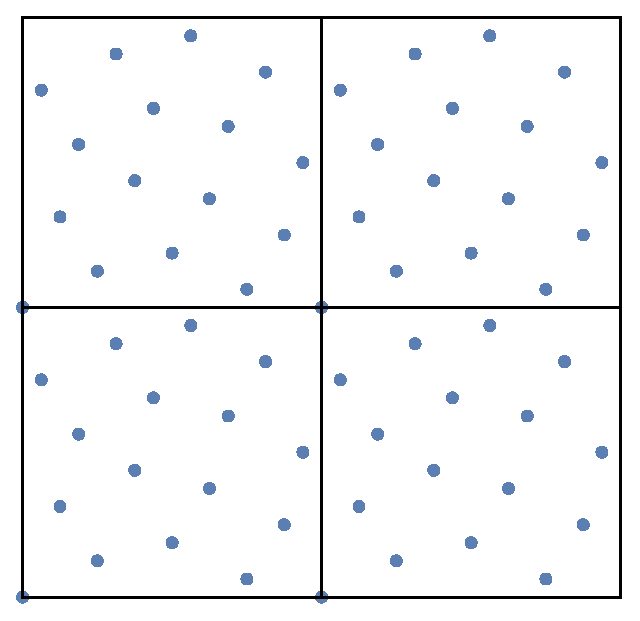
\includegraphics[width=0.5\linewidth]{chap07/maxmin2x2pix.eps}
    \caption{$2\times2$像素网格,每个都用来自\refvar{MaxMinDistSampler}{}的16个样本采样。
        尽管每个像素用相同的采样点,但已经优化了其摆放使得它们不仅在每个像素内分布良好,
        而且在它们跨像素铺展时样本点也不会太靠近相邻像素中的点。}
    \label{fig:7.33}
\end{figure}

\begin{lstlisting}
`\refcode{Low Discrepancy Declarations}{+=}\lastnext{LowDiscrepancyDeclarations}`
extern uint32_t `\initvar{CMaxMinDist}{}`[17][32];
\end{lstlisting}

\refvar{MaxMinDistSampler}{}使用生成矩阵来计算像素样本。
2D样本第一维的值通过在第一维内均匀步进来设置,第二维来自生成矩阵。
\begin{lstlisting}
`\initcode{MaxMinDistSampler Method Definitions}{=}`
void `\refvar{MaxMinDistSampler}{}`::`\initvar[MaxMinDistSampler::StartPixel]{StartPixel}{}`(const `\refvar{Point2i}{}` &p) {
    `\refvar{Float}{}` invSPP = (`\refvar{Float}{}`)1 / `\refvar{samplesPerPixel}{}`;
    for (int i = 0; i < `\refvar{samplesPerPixel}{}`; ++i)
        `\refvar{samples2D}{}`[0][i] = `\refvar{Point2f}{}`(i * invSPP, 
                                  `\refvar{SampleGeneratorMatrix}{}`(`\refvar{CPixel}{}`, i));
    `\refvar{Shuffle}{}`(&`\refvar{samples2D}{}`[0][0], `\refvar{samplesPerPixel}{}`, 1, `\refvar[PixelSampler::rng]{rng}{}`);
    `\refcode{Generate remaining samples for MaxMinDistSampler}{}`
    `\refvar{PixelSampler}{}`::StartPixel(p);
}
\end{lstlisting}

剩下的维度用前两个Sobol矩阵采样,就像\refvar{ZeroTwoSequenceSampler}{}那样。
(比起用矩阵\refvar{CMaxMinDist}{})我们对样本向量的非图像维度使用该方法求得了稍好的结果。
因此,这里没有介绍相应的代码片{\refcode{Generate remaining samples for MaxMinDistSampler}{}}
\sidenote{译者注:我补充回来了。}。
\begin{lstlisting}
`\initcode{Generate remaining samples for MaxMinDistSampler}{=}`
for (size_t i = 0; i < `\refvar{samples1D}{}`.size(); ++i)
    `\refvar{VanDerCorput}{}`(1, `\refvar{samplesPerPixel}{}`, &`\refvar{samples1D}{}`[i][0], `\refvar[PixelSampler::rng]{rng}{}`);

for (size_t i = 1; i < `\refvar{samples2D}{}`.size(); ++i)
    `\refvar{Sobol2D}{}`(1, `\refvar{samplesPerPixel}{}`, &`\refvar{samples2D}{}`[i][0], `\refvar[PixelSampler::rng]{rng}{}`);

for (size_t i = 0; i < `\refvar{samples1DArraySizes}{}`.size(); ++i) {
    int count = `\refvar{samples1DArraySizes}{}`[i];
    `\refvar{VanDerCorput}{}`(count, `\refvar{samplesPerPixel}{}`, &`\refvar{sampleArray1D}{}`[i][0], `\refvar[PixelSampler::rng]{rng}{}`);
}

for (size_t i = 0; i < `\refvar{samples2DArraySizes}{}`.size(); ++i) {
    int count = `\refvar{samples2DArraySizes}{}`[i];
    `\refvar{Sobol2D}{}`(count, `\refvar{samplesPerPixel}{}`, &`\refvar{sampleArray2D}{}`[i][0], `\refvar[PixelSampler::rng]{rng}{}`);
}
\end{lstlisting}